\documentclass{beamer}
%
% Choose how your presentation looks.
%
% For more themes, color themes and font themes, see:
% http://deic.uab.es/~iblanes/beamer_gallery/index_by_theme.html
%
\mode<presentation>
{
  \usetheme{boxes}      % or try Darmstadt, Madrid, Warsaw, ...
  \usecolortheme{dove} % or try albatross, beaver, crane, ...
  \usefonttheme{structurebold}  % or try serif, structurebold, ...
  \setbeamertemplate{navigation symbols}{}
  \setbeamertemplate{caption}[numbered]
} 

\usepackage[english]{babel}
\usepackage[utf8x]{inputenc}

\title[Your Short Title]{GPU-Accelerated Deep Neural Networks in TMVA}
\date{}
\author{Simon Pfreundschuh  \\ \textbf{Supervisors}: Sergei V. Gleyzer, Lorenzo Moneta}
\titlegraphic{
\includegraphics[width=0.2\textwidth]{gsoc}%
              \hskip 2cm 
\includegraphics[width=0.2\textwidth]{cern}}
\begin{document}
\addtobeamertemplate{navigation symbols}{}{ \hspace{1em}    \usebeamerfont{footline}%
    \insertframenumber / \inserttotalframenumber }
\begin{frame}
  \titlepage
\end{frame}

% Uncomment these lines for an automatically generated outline.
\begin{frame}{Outline}
 \tableofcontents
\end{frame}
\AtBeginSection[]{
  \begin{frame}
  \vfill
  \centering
  \begin{beamercolorbox}[sep=8pt,center,shadow=true,rounded=true]{title}
    \usebeamerfont{title}\insertsectionhead\par%
  \end{beamercolorbox}
  \vfill
  \end{frame}
}
\setbeamertemplate{itemize items}[circle]
\section{Introduction}

\begin{frame}{Motivation}
  \begin{itemize}
    \item Deep learning techniques have been revolutionizing
      the field of machine learning.
    \item Their success is closely related to the development of
      massively parallel accelerator devices, which allow for efficient
      training of machine learning models.
    \item Deep learning techniques have successfully been applied to
      problems in HEP\footnote{\url{http://arxiv.org/pdf/1402.4735v2.pdf}}.
  \end{itemize}
  \visible<2->{
  \begin{block}{Aim}
    Provide an efficient and easy-to-use implementation of deep neural
    networks for the HEP community.
  \end{block}
  }
\end{frame}

\begin{frame}{TMVA}
  \begin{itemize}
    \item Toolkit for Multivariate Data Analysis with ROOT
    \item Root-integrated machine learning (ML) environment providing
      a training and test framework for a large number of ML methods.
  \end{itemize}
  \vfill
  \centering
  
\includegraphics[width=0.5\linewidth]{tmva}
\end{frame}

\begin{frame}{Feed Forward Neural Networks}

  \begin{overprint}
  \onslide<1>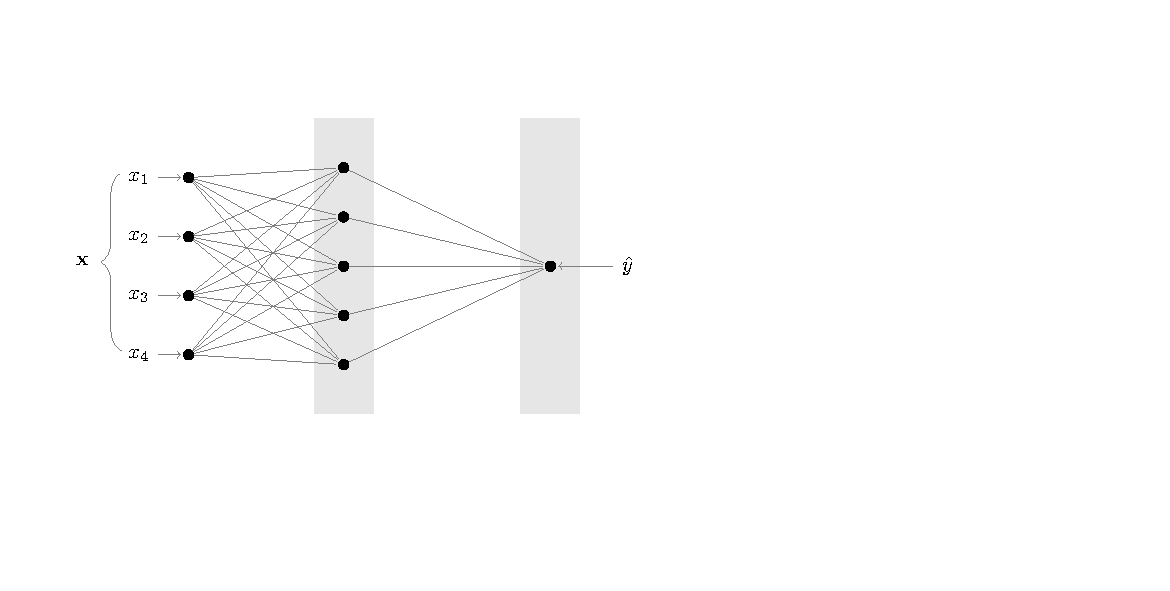
\includegraphics[ width=1.1\linewidth]{nn_1}
  \onslide<2>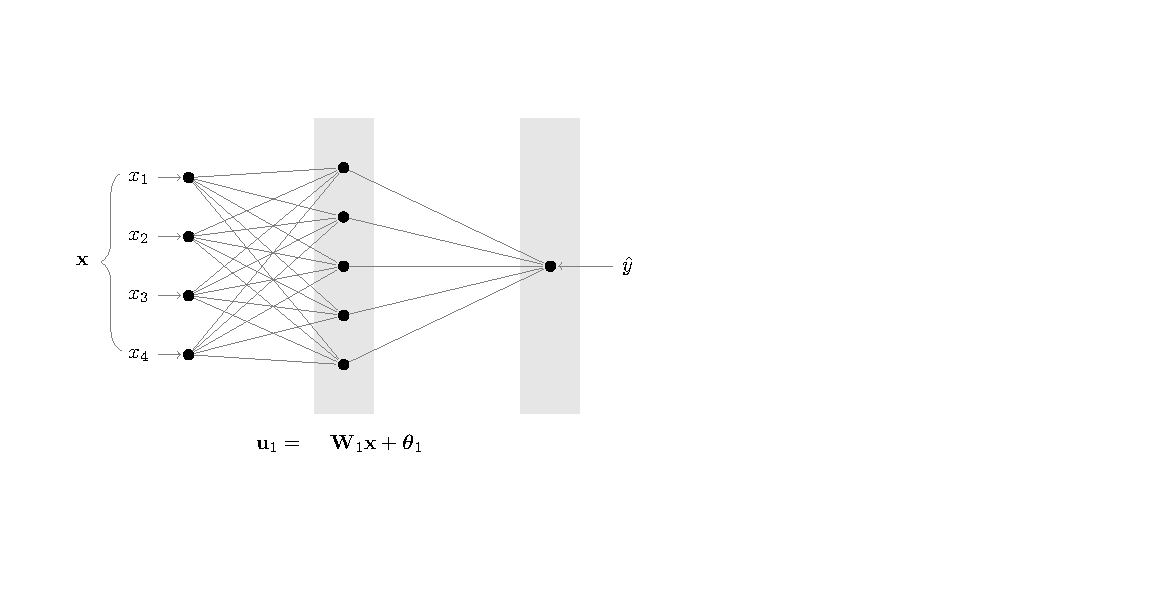
\includegraphics[ width=1.1\linewidth]{nn_2}
  \onslide<3>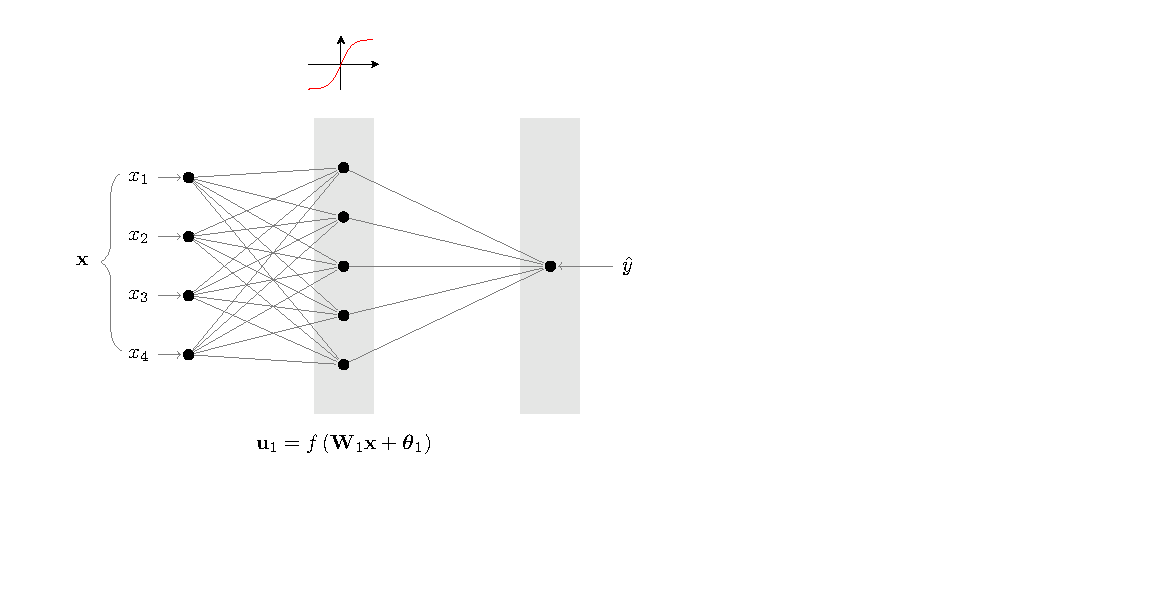
\includegraphics[ width=1.1\linewidth]{nn_3}
  \onslide<4>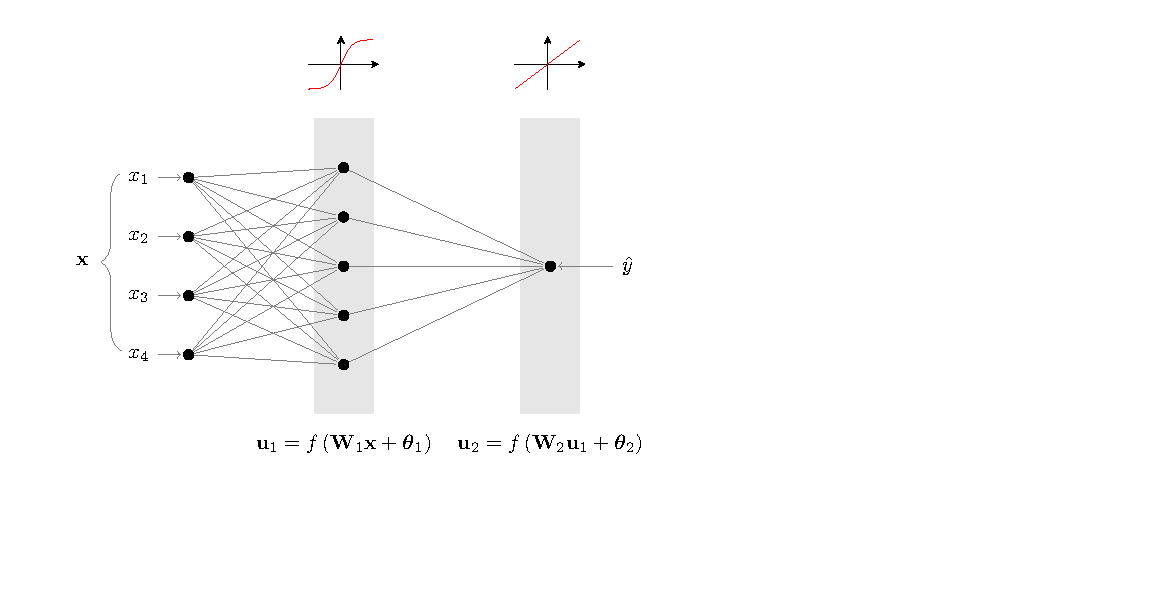
\includegraphics[ width=1.1\linewidth]{nn_4}
  \onslide<5>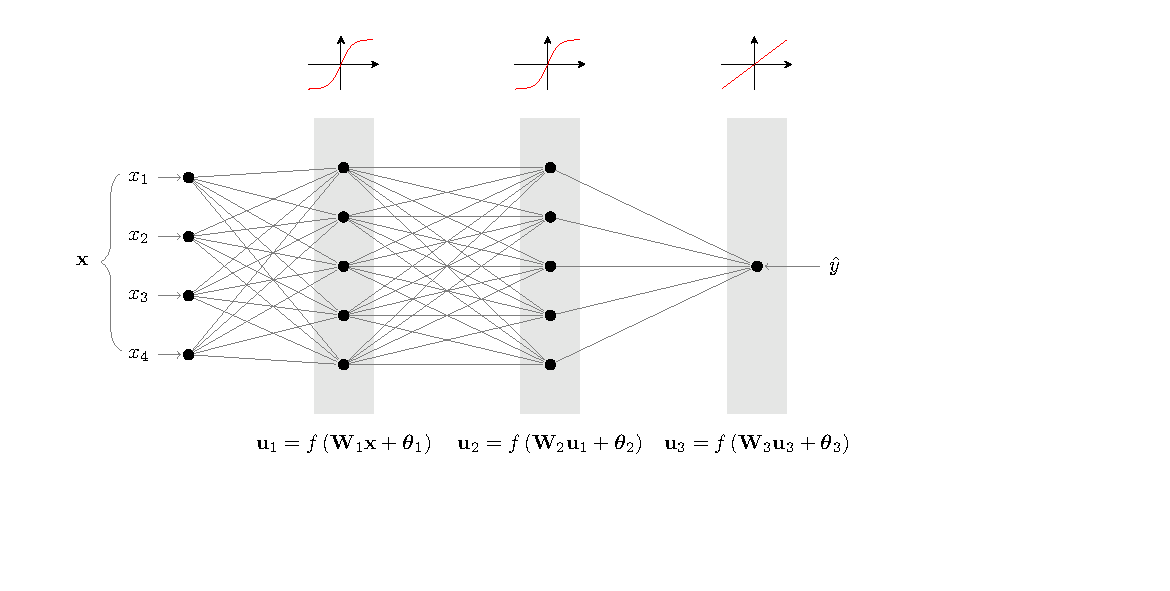
\includegraphics[ width=1.1\linewidth]{nn_5}
  \onslide<6>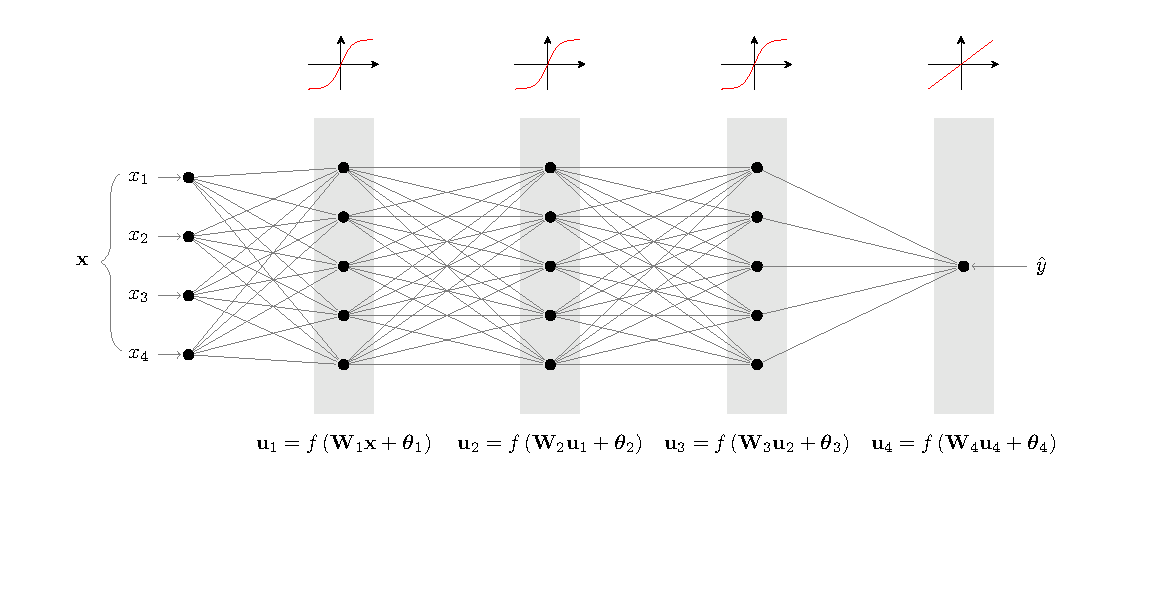
\includegraphics[ width=1.1\linewidth]{nn_6}
  \onslide<7>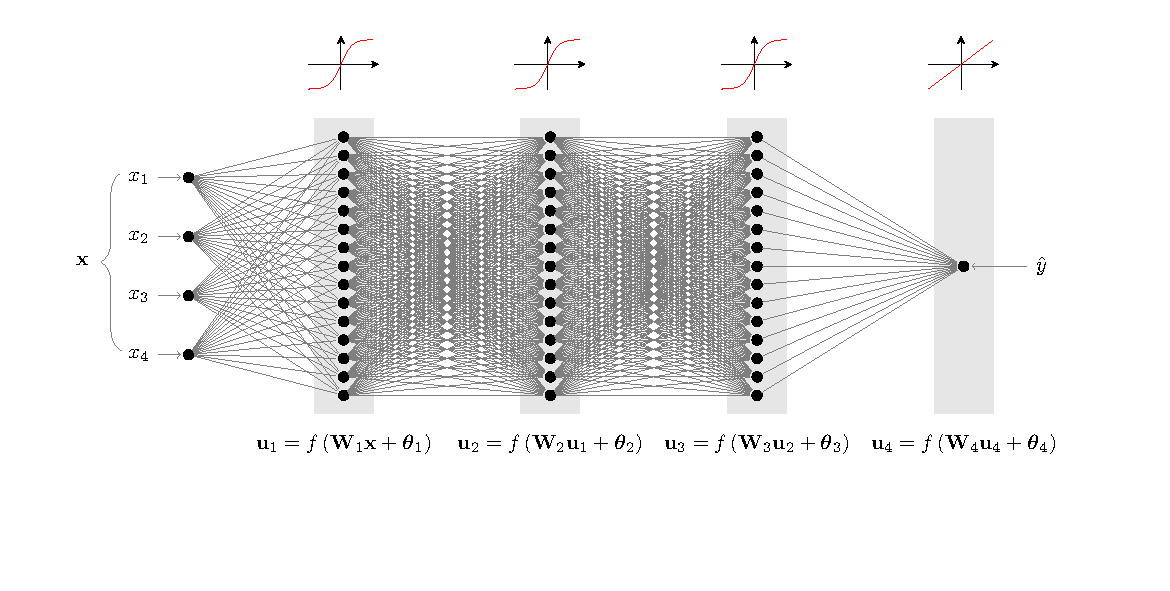
\includegraphics[ width=1.1\linewidth]{nn_7}
  \end{overprint}

\end{frame}

\begin{frame}{Feed Forward Neural Networks}
  \begin{itemize}
  \item A feed forward neural network is defined by a set of layers $l=1,\ldots,n$,
    each with an associated weight matrix $\mathbf{W}_l$, bias terms
    $\mathbf{\theta}_l$ and activation function $f_l$.
  \item \textbf{Feed forward}: Neurons of a given layer $l$ are only connected to neurons of the layer $l + 1$
  \item A neural network may be viewed as a function
    \begin{align}
      F(\mathbf{x}, \mathbf{W}, \boldsymbol{\theta}) &=
      f_{n}\left(f_{n-1}(\cdots)\mathbf{W}_{n-1}^T + \boldsymbol{\theta}_{n-2}\right) \mathbf{W}_n^T + \boldsymbol{\theta}_n
    \end{align}
  \item<2> \textbf{Machine Learning}: Find parameters $\hat{\mathbf{W}},
    \hat{\boldsymbol{\theta}}$ so that
    $F(\mathbf{x}) = F(\mathbf{x}, \hat{\mathbf{W}}, \hat{\boldsymbol{\theta}})$
    approximates either a target function $G(\mathbf{x})$ (\textbf{Regression}) or
    a likelihood measure for a given class (\textbf{Classification}).
    \end{itemize}

\end{frame}
\begin{frame}{Neural Network Training}
  \begin{itemize}
  \item \textbf{Supervised learning}: The network is trained using a training
  set consisting of inputs $\mathcal{X} = {\mathbf{x}_0,\ldots,\mathbf{x}_n}$
  and outputs $\mathcal{Y} = {y_0,\ldots,y_n}$.
  \item The \textbf{loss function} or \textbf{error function}
  $J(y, \hat{y})$ quantifies the quality of
    a prediction $\hat{y}$ with respect to the expected output $y$.
  \item Learning as a minimization problem:
    \begin{align}
      \underset{\mathbf{W},\boldsymbol{\theta}}{\text{minimize }}
         J_\mathcal{X} = \frac{1}{n}\sum_{\mathbf{x}} J(y, \hat{y})
      \end{align}
 \end{itemize}
 \end{frame}


\begin{frame}{Neural Network Training (Contd.)}
  \begin{itemize}
    \item Use gradient-based minimization methods to minimize
      the error $\sum_{\mathbf{x} \in \mathcal{X}}J(y,\hat{y})$ over the training set:

      \begin{align}
        \mathbf{W} \leftarrow \mathbf{W} - \alpha \frac{dJ_\mathcal{X}}{d\mathbf{W}} \\
        \boldsymbol{\theta} \leftarrow \boldsymbol{\theta} - \alpha 
\frac{d J_\mathcal{X}}{d\boldsymbol{\theta}}
        \end{align}
   \item \textbf{Batch gradient descent}: Instead of the whole training set,
     compute the gradient only for a small subset of it.
   \item Crucial for scalable training on large data sets.

 \end{itemize}
\end{frame}

\begin{frame}{Forward and Backward Propagation}
  \textbf{Forward Propagation:}
    \begin{align}
      \mathbf{U}_n &= f_n\left ( \mathbf{U}_{n-1} \mathbf{W}_n
                              + \boldsymbol{\theta}^T \right) \\
              \mathbf{f}'_n &= f'_n\left ( \mathbf{U}_{n-1} \mathbf{W}_n
                              + \boldsymbol{\theta}^T \right) 
      \end{align}
 \textbf{Backward Propagation:}
    \begin{align}
      \frac{dJ_\mathcal{X}}{d\mathbf{W}_n} &=  \mathbf{U}_{n-1} \left(\mathbf{f}'_n \odot 
           \frac{dJ_\mathcal{X}}{d\mathbf{U}_n} \right)  \\
      \frac{dJ_\mathcal{X}}{d\boldsymbol{\theta}_n} &=  \mathbf{1} \left(\mathbf{f}'_n \odot 
           \frac{dJ_\mathcal{X}}{d\mathbf{U}_n} \right) \\
      \frac{dJ_\mathcal{X}}{d\mathbf{U}_{n-1}} &=  \mathbf{W}_n \left(\mathbf{f}'_n \odot 
           \frac{dJ_\mathcal{X}}{d\mathbf{U}_n} \right)
      \end{align}
\end{frame}

\begin{frame}{Forward and Backward Propagation}

  \begin{overprint}
  \onslide<1>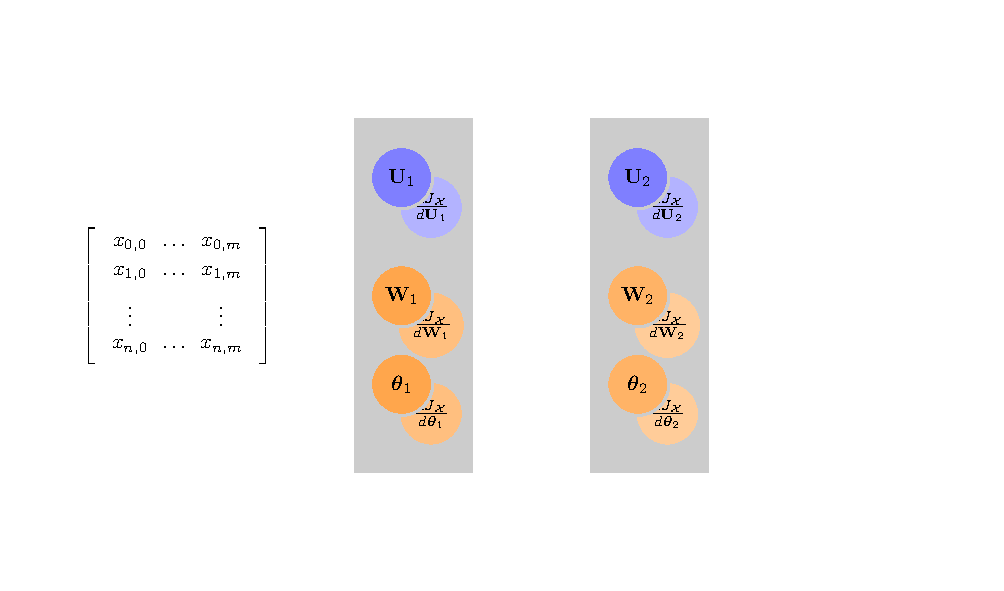
\includegraphics[ width=1.1\linewidth]{backprop_0}
  \onslide<2>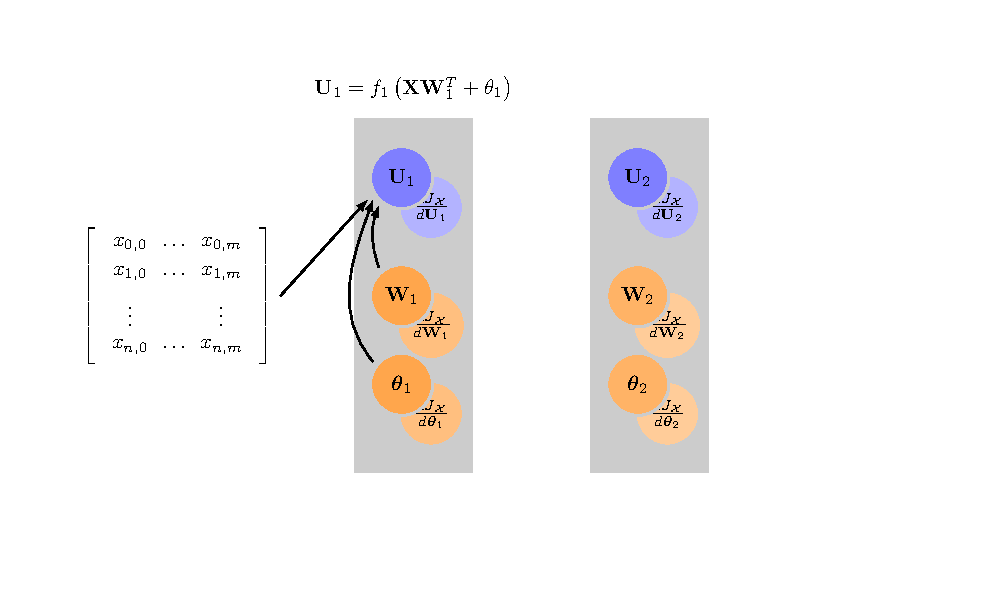
\includegraphics[ width=1.1\linewidth]{backprop_1}
  \onslide<3>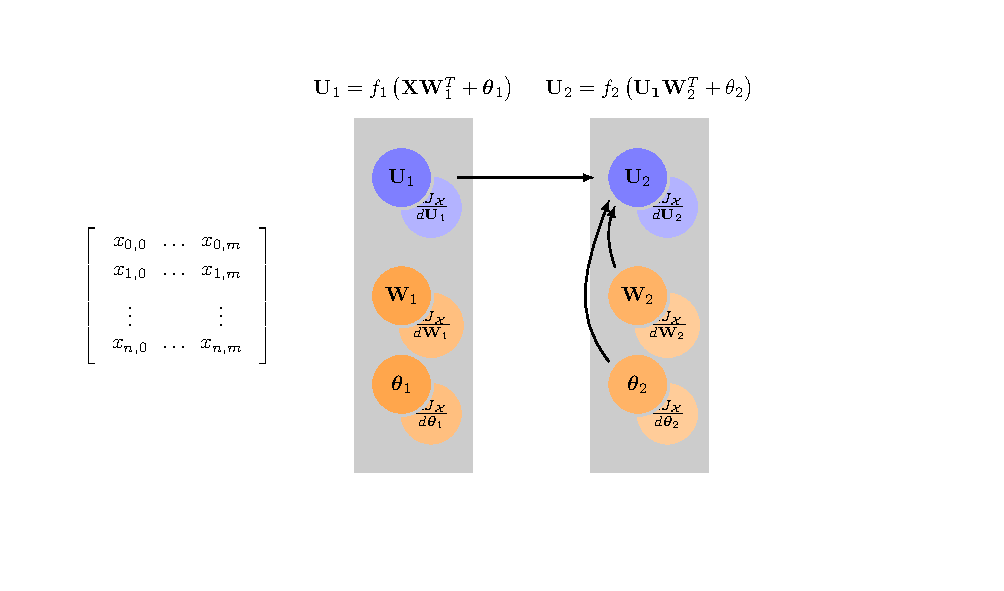
\includegraphics[ width=1.1\linewidth]{backprop_2}
  \onslide<4>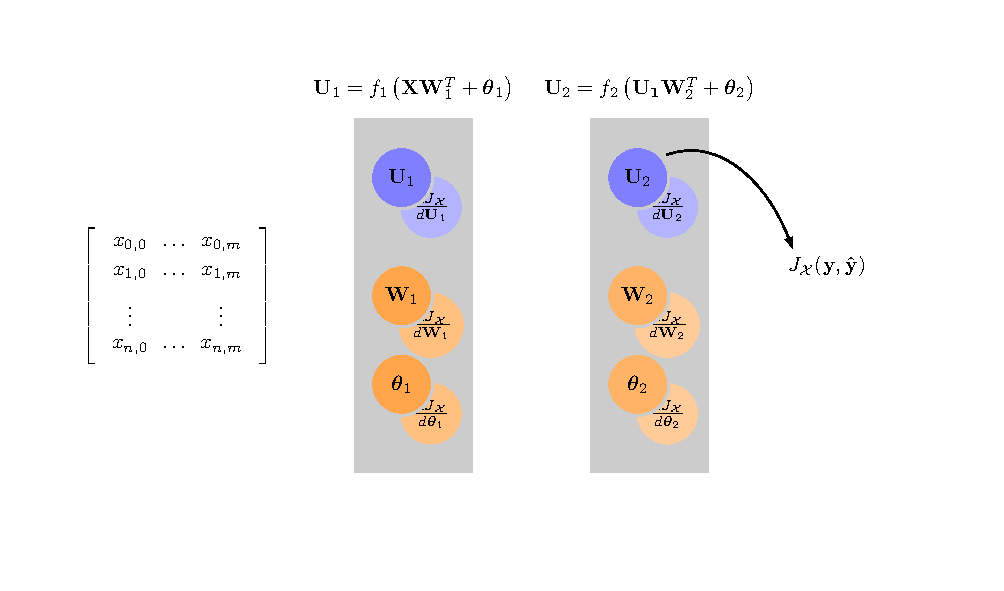
\includegraphics[ width=1.1\linewidth]{backprop_3}
  \onslide<5>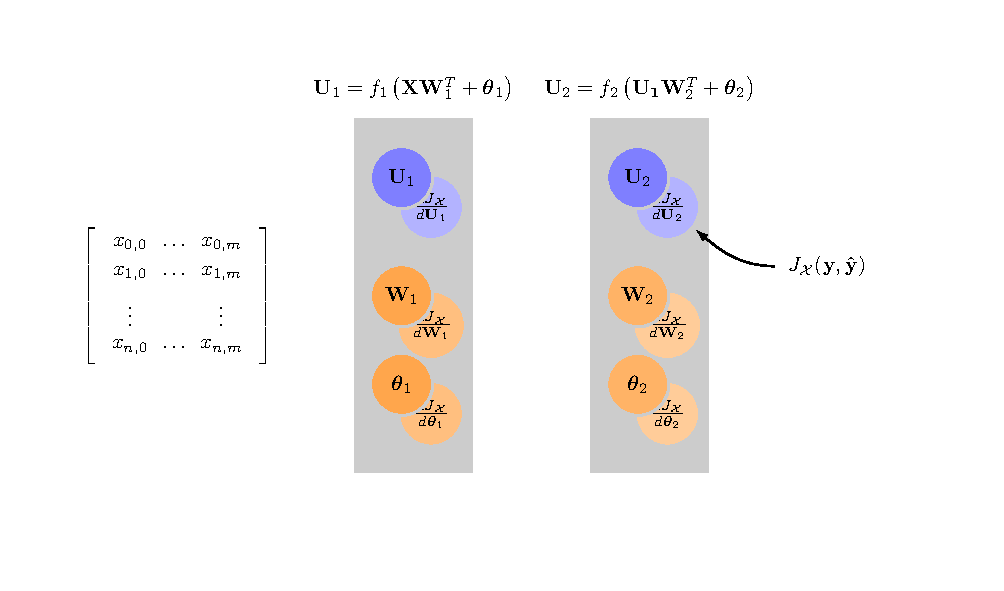
\includegraphics[ width=1.1\linewidth]{backprop_4}
  \onslide<6>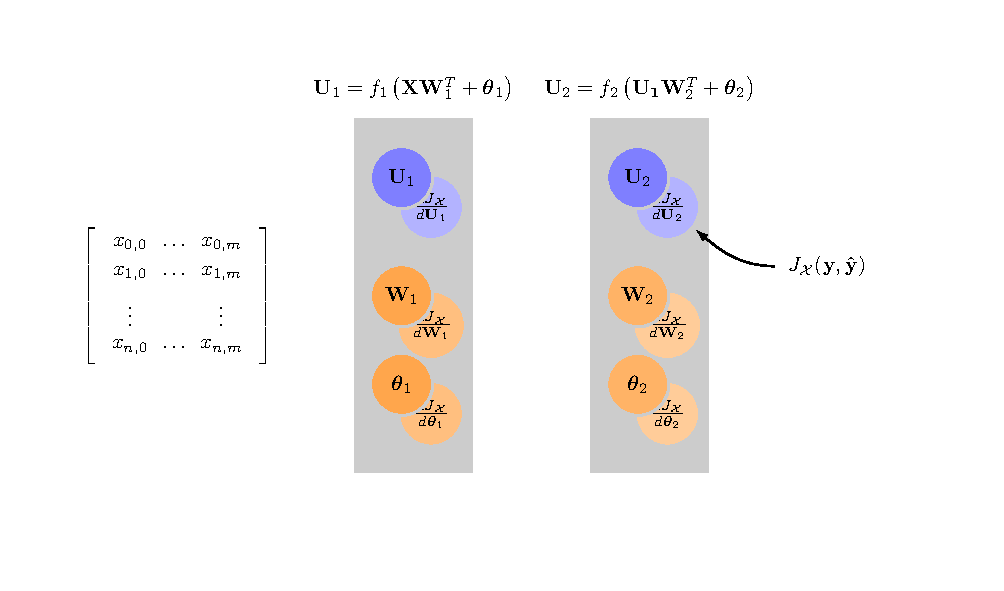
\includegraphics[ width=1.1\linewidth]{backprop_5}
  \onslide<7>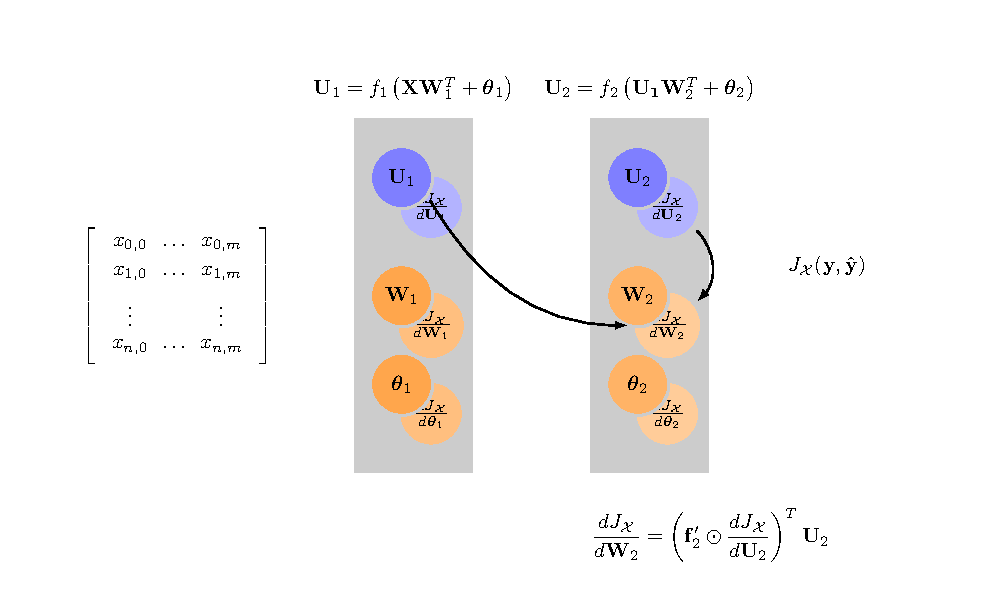
\includegraphics[ width=1.1\linewidth]{backprop_6}
  \onslide<8>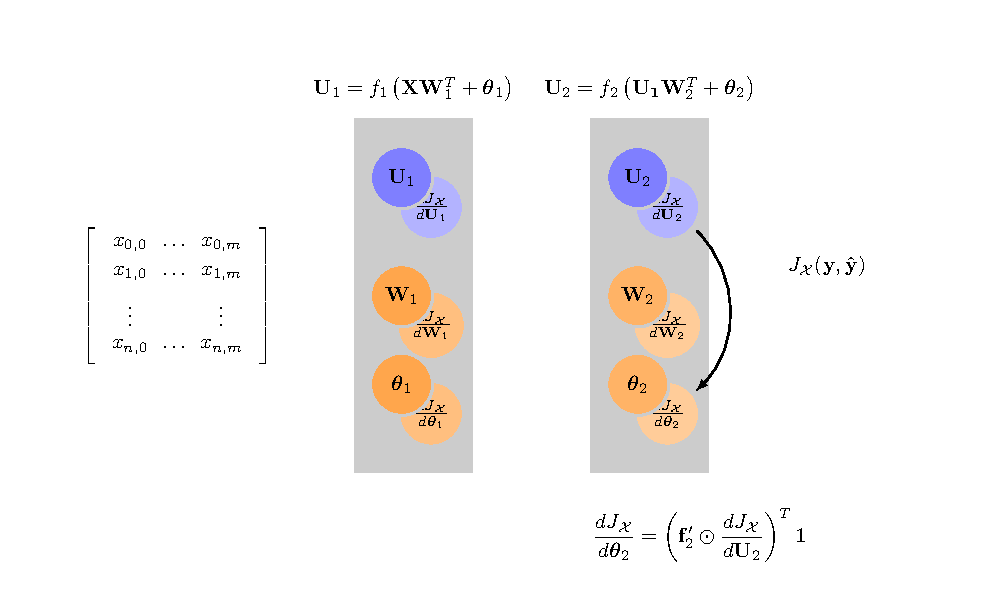
\includegraphics[ width=1.1\linewidth]{backprop_7}
  \onslide<9>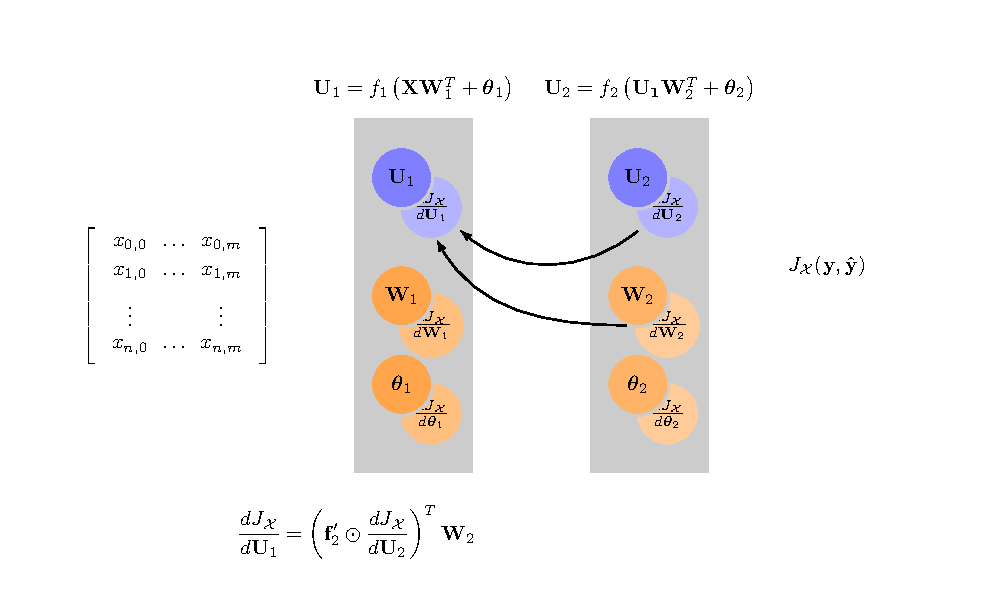
\includegraphics[ width=1.1\linewidth]{backprop_8}
  \onslide<10>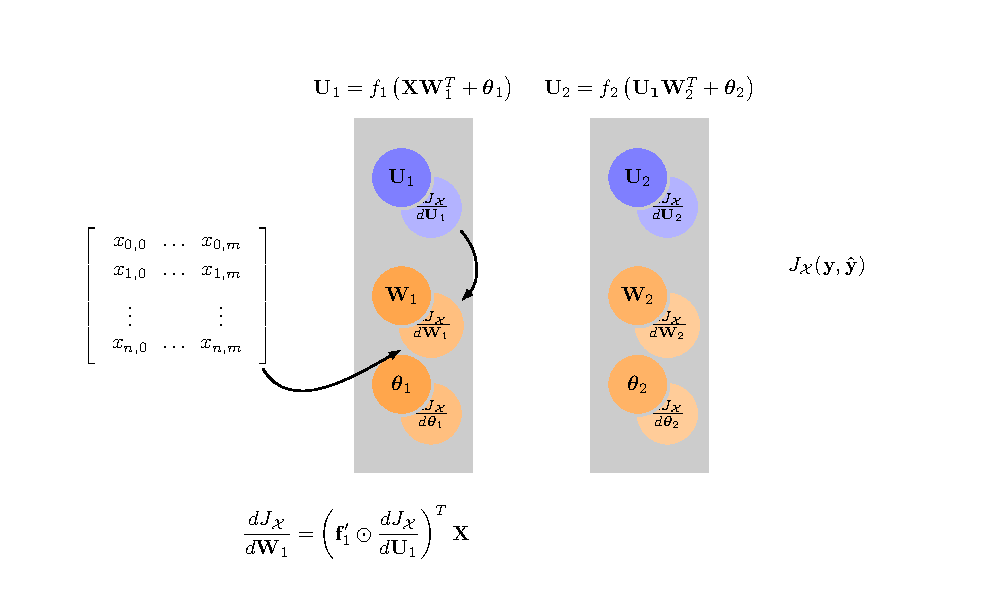
\includegraphics[ width=1.1\linewidth]{backprop_9}
  \onslide<11>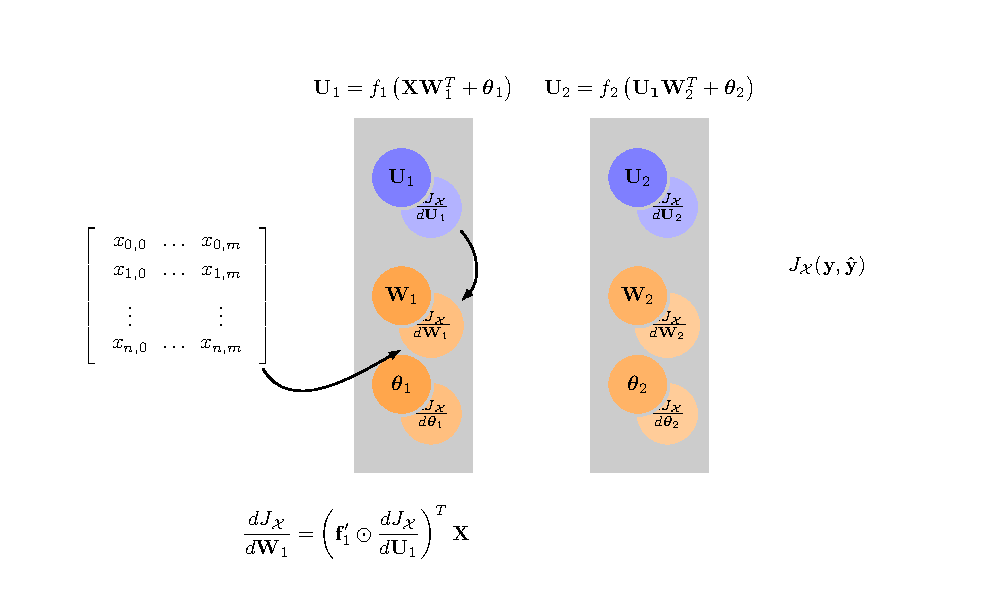
\includegraphics[ width=1.1\linewidth]{backprop_10}
  \onslide<12>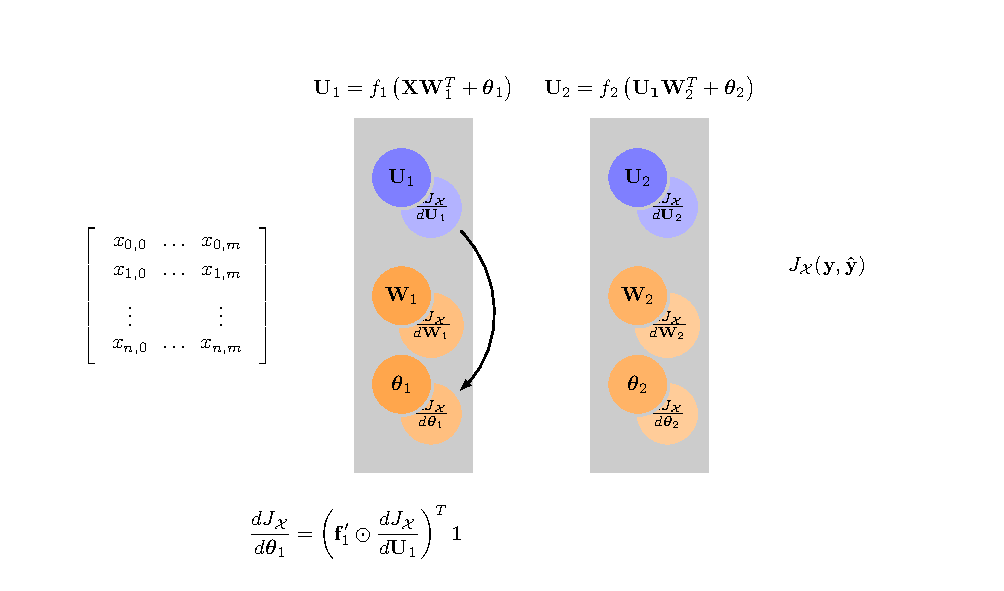
\includegraphics[ width=1.1\linewidth]{backprop_11}
  \end{overprint}

\end{frame}
\section{Implementation}

\begin{frame}{Design}
  \begin{itemize}
    \item The backpropagation algorithm can be decomposed into primitive operations
      on matrices:
      \begin{itemize}
        \item Matrix multiplication and addition
        \item Application of activation functions
        \item Computing of loss and regularization functionals
        \end{itemize}
   \item General formulation of the backpropagation algorithm using
     those primitive matrix operations
   \item Optimized matrix operations provided by specialized low-level implementations
   \end{itemize}
 \end{frame}

\begin{frame}{Design}
  \begin{overprint}
  \onslide<1>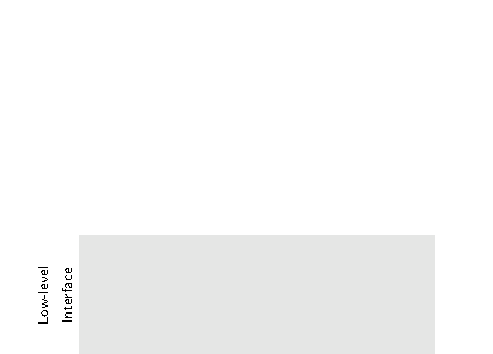
\includegraphics[ width=1.1\linewidth]{struct_0}
  \onslide<2>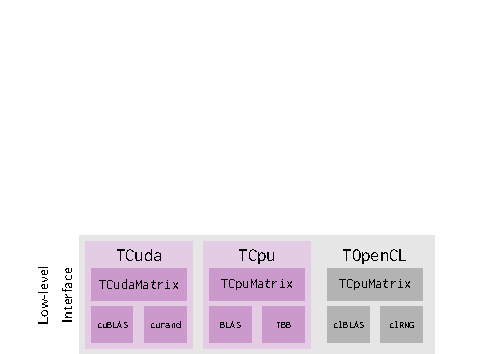
\includegraphics[ width=1.1\linewidth]{struct_1}
  \onslide<3>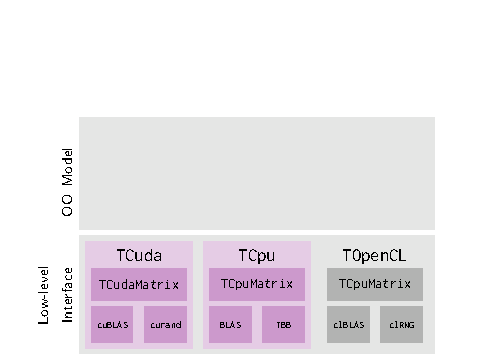
\includegraphics[ width=1.1\linewidth]{struct_2}
  \onslide<4>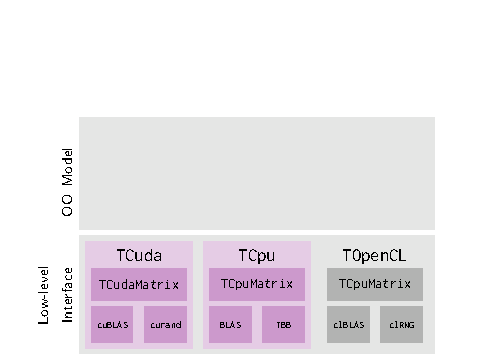
\includegraphics[ width=1.1\linewidth]{struct_3}
  \onslide<5>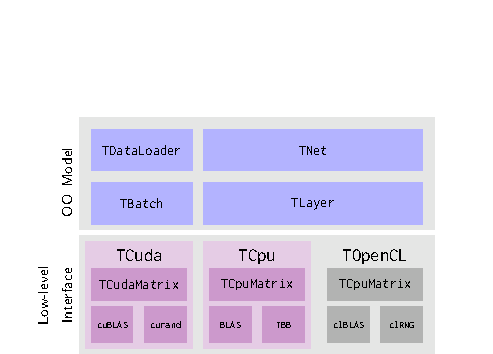
\includegraphics[ width=1.1\linewidth]{struct_4}
  \onslide<6>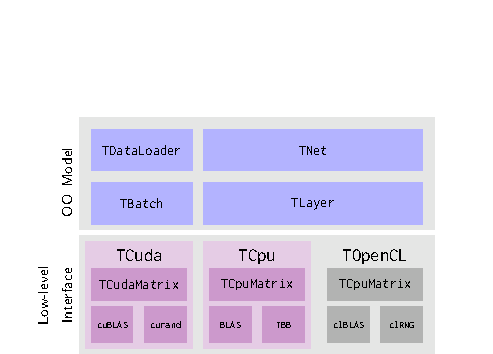
\includegraphics[ width=1.1\linewidth]{struct_5}
  \onslide<7>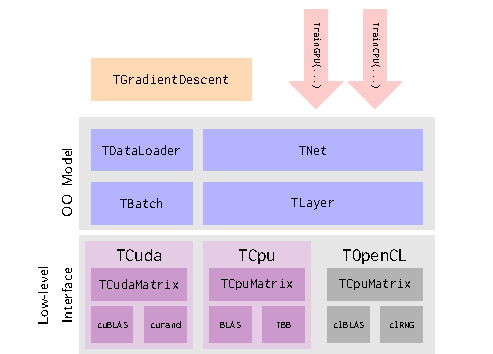
\includegraphics[ width=1.1\linewidth]{struct_6}
  \end{overprint}

\end{frame}

\begin{frame}{Design}
  \textbf{The Low-Level Interface:}
  \begin{itemize}
    \item Implemented by architecture classes: \texttt{TCuda, TCpu, TOpenCL}
    \item Architecture classes provide \textbf{matrix} and \textbf{scalar} types
      as well as \textbf{host} and \textbf{device} buffer types
  \end{itemize}
  \textbf{The Object Oriented Model:}
 \begin{itemize}
    \item Generic neural network implementation: Classes are templated
     by architecture class.
    \item The \texttt{TNet} class provides a general implementation of the
      backpropagation algorithm.
    \item The \texttt{TDataLoader} takes care of the streaming of data to
      the device.
 \end{itemize}
\end{frame}

\begin{frame}{Dependencies}
  \textbf{CPU Implementation}:
  \begin{itemize}
    \item BLAS: quasi-standard, various optimized free-software
      implementations available, possibility to link againt vendor provided
      implementation when available
    \item TBB: Considered using Root's ThreadPool, but lacks block range
      functionality
  \end{itemize}
  \visible<2>{
  \textbf{CUDA Implementation}:
  \begin{itemize}
  \item There exist dedicated neural network libraries developed by NVIDIA
    but obtaining them requires joining \textit{Accelerated Computing Developer Program}
  \item cuBLAS and cuRAND freely available as part of the CUDA Toolkit
  \end{itemize}
  }
\end{frame}
\begin{frame}{Dependencies}
  \textbf{OpenCL Implementation}:
  \begin{itemize}
    \item clBLAS: Part of the open-source clMath\footnote{\url{https://github.com/clMathLibraries}} libraries
    \item clRNG: Also part of the clMath libraries
    \item Encountered portability problems with the clRNG library.
  \end{itemize}
\end{frame}

\section{Verification and Testing}

\begin{frame}{Verification}
\begin{itemize}
  \item Backpropagation algorithm verified using \textbf{numerical differentiation}.
  \item Weight gradient error for a network with sigmoid activations (foreground)
    and identity activations (background):
  \item The code includes a reference low-level implementation based on
    Root's \texttt{TMatrix} class.
  \item Generic unit test for all routines in the low-level interface based
    on the reference implementation.
  \item Training routines verified by learning full-rank linear mappings.
    \end{itemize}
\end{frame}
\section{Performance}
\begin{frame}{Performance Model}
  Consider a layer $l$ with $n_l$ neurons, $n_{l-1}$ input neurons and a batch
  size of $n_b$.
  \begin{overprint}
  \onslide<1>%
  \begin{block}{Forward Propagation:}
    \begin{itemize}
    \item Multiplication of weight matrix $\mathbf{W}_l$ with activation gradients:
      \begin{align*}
n_l n_b (2n_{l-1} - 1) \: \text{ FLOP}
        \end{align*}
    \item Addition of bias terms $\boldsymbol{\theta}_l$:
      \begin{align*}
      n_l n_b \:  \text{ FLOP}
        \end{align*}
    \item Application of activation function $f_l$ and its derivatives:
   \begin{align*}
     2 n_l n_b c_f \:\text{ FLOP}, \quad c_f \approx 1
   \end{align*}
     \end{itemize}
   \end{block}
   \onslide<2>
   \begin{block}{Backward Propagation}
    \begin{itemize}
    \item Hadamard product:
      \begin{align*}
        n_l n_b \: \text{ FLOP}
      \end{align*}
    \item Computation of previous layer activations:
      \begin{align*}
        n_{l-1} n_b (2 n_l - 1) \: \text{ FLOP}
      \end{align*}
    \item Computation of weight and bias gradients:
      \begin{align*}
        n_{l-1} n_l (2 n_b - 1) + n_l(n_b - 1) \: \text{ FLOP}
      \end{align*}
   \end{itemize}
   \end{block}
   \onslide<3>
   \begin{block}{Total:}
      \begin{align*}
 \sum_l 6n_l n_b n_{l-1}  + 4 n_l n_b - n_l(n_{l-1} + 1) - n_bn_{l-1} 
      \end{align*}
      \begin{itemize}
      \item Terms involving $n_l n_b n_{l-1}$ dominate complexity for the \textit{hidden}
        layers.
      \end{itemize}
    \end{block}
  \end{overprint}
\end{frame}

\begin{frame}{Benchmarks}
  \begin{itemize}
    \item Training Data:
      \begin{itemize}
      \item Randomly generated data from a linear mapping
        $\mathrm{R}^{20} \mapsto \mathrm{R}$
      \item $10^5$ input samples
        \end{itemize}
       \item Computation of the numerical throughput based on the time elapsed
         for performing 10 training epochs.
      \item Network structure:
        \begin{itemize}
          \item 5 hidden layers with 256 neurons
          \item $tanh$ activation functions
          \item Sqaured error loss
          \end{itemize}
    \end{itemize}
\end{frame}

\begin{frame}{CPU Performance}
  \textbf{Implementation}: Multithreaded OpenBLAS  and TBB \\
  \textbf{Hardware}: Intel Xeon E5-2650, $8 \times 4$ cores, $2\: GHz$,
  estimated peak performance per core: $16$ GFLOP/s
   \centering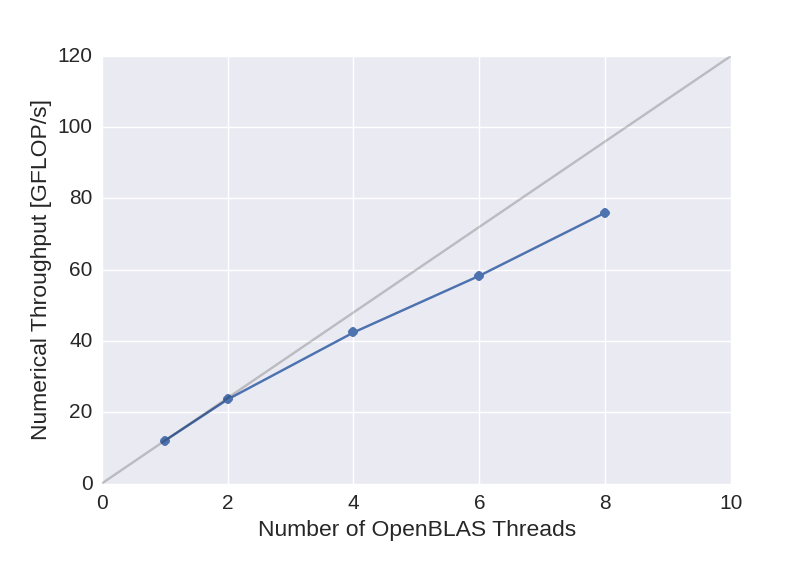
\includegraphics[ width=0.7\linewidth]{perf_cpu}
\end{frame}

\begin{frame}{GPU Performance}
  \textbf{Network}: 20 input nodes, 5 hidden layers with $n_h$ nodes each,
  squared error loss \\
  \textbf{Hardware}: NVIDIA Tesla K20, $1.17$ TFLOP/s peak performance (double)

  \begin{center}
  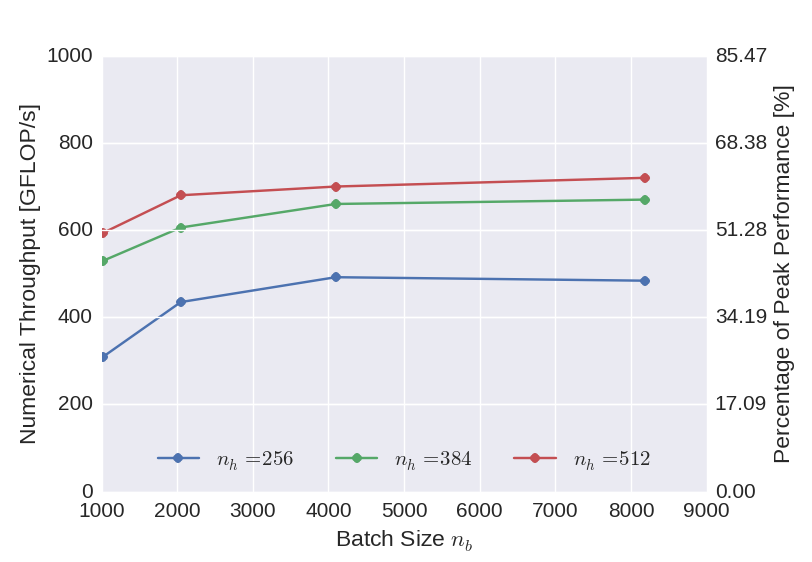
\includegraphics[width=0.7\linewidth]{perf_gpu}
  \end{center}

\end{frame}
\begin{frame}{GPU Performance}
  \textbf{Optimization}:
  \begin{itemize}
    \item Use compute streams to expose more parallelism to the device.
    \item Compute gradients for multiple batches in parallel.
      \begin{overprint}
        \onslide<2>\item Using 2 streams:
        \onslide<3>\item Using 4 streams:
      \end{overprint}
  \end{itemize}
  \begin{center}
  \begin{overprint}
  \onslide<2>\centering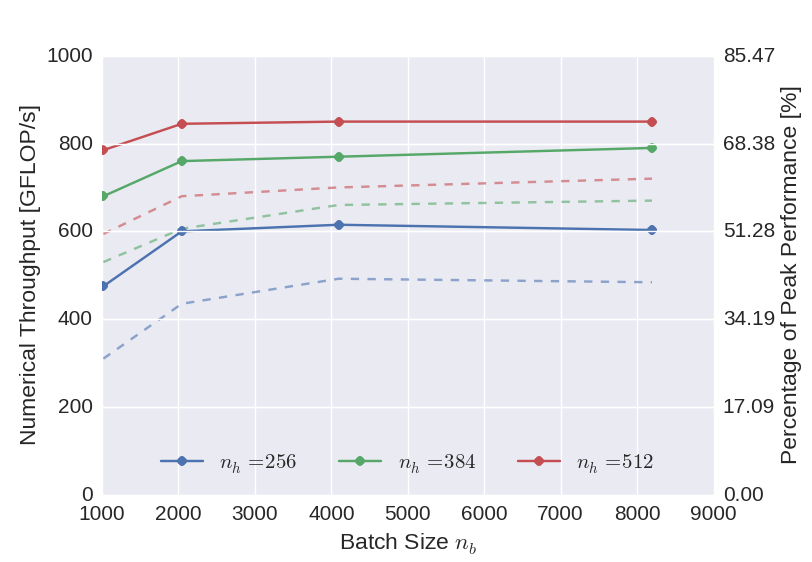
\includegraphics[ width=0.7\linewidth]{perf_2_gpu}
  \onslide<3>\centering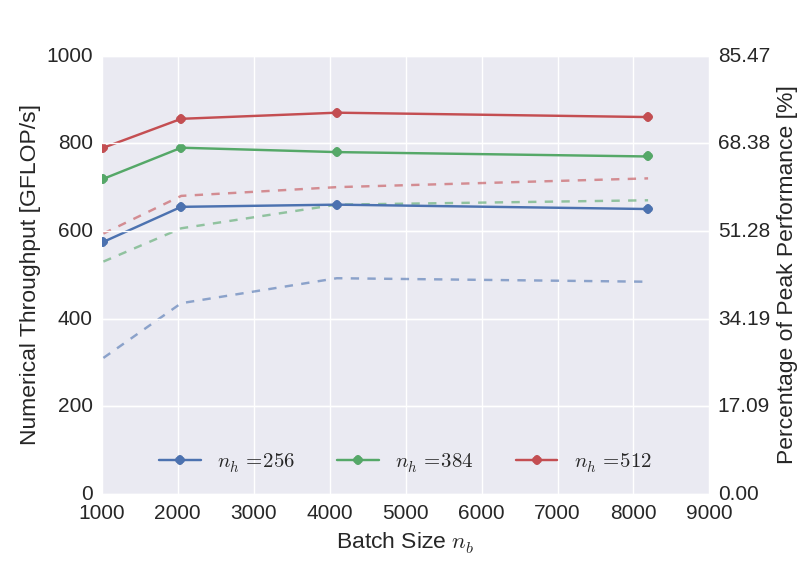
\includegraphics[ width=0.7\linewidth]{perf_3_gpu}
  \end{overprint}
  \end{center}
\end{frame}

\begin{frame}{GPU Performance}
  \textbf{Network}: 20 input nodes, 5 hidden layers with $256$ nodes each,
  squared error loss \\
  \textbf{Hardware}: NVIDIA Tesla K20, $1.17$ TFLOP/s peak performance (double)
  \begin{center}
  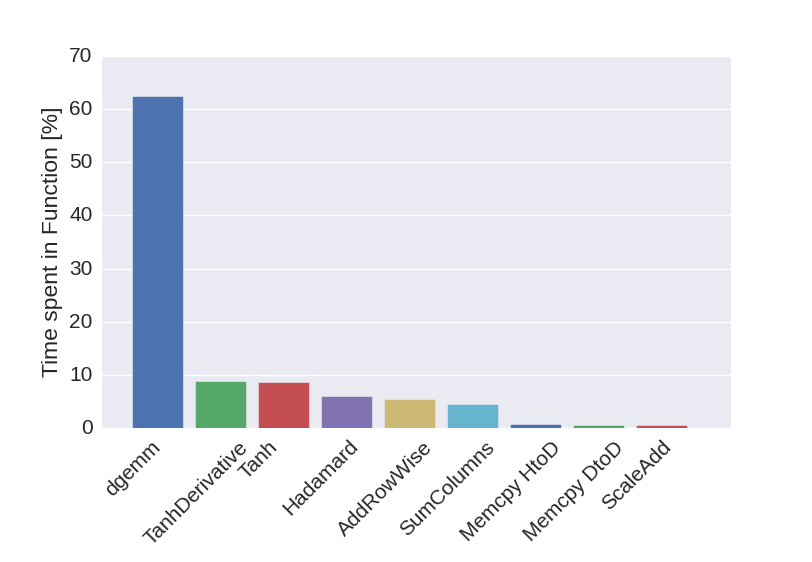
\includegraphics[width=0.8\linewidth]{prof_gpu}
  \end{center}
\end{frame}

\begin{frame}{OpenCL Performance}
  \textbf{Network}: 20 input nodes, 5 hidden layers with $256$ nodes each,
  squared error loss \\
  \textbf{Hardware}: AMD FirePro W8100, $2.1$ TFLOP/s peak performance (double)
  \begin{center}
  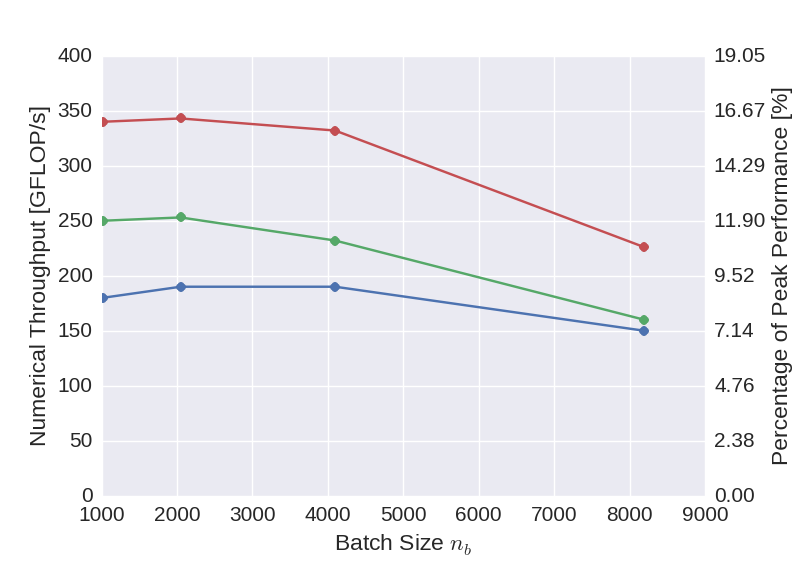
\includegraphics[width=0.8\linewidth]{perf_opencl}
  \end{center}
\end{frame}

\begin{frame}{Summary}
  \textbf{Network}: 20 input nodes, 5 hidden layers with $256$ nodes each,
  squared error loss \\
  \begin{center}
  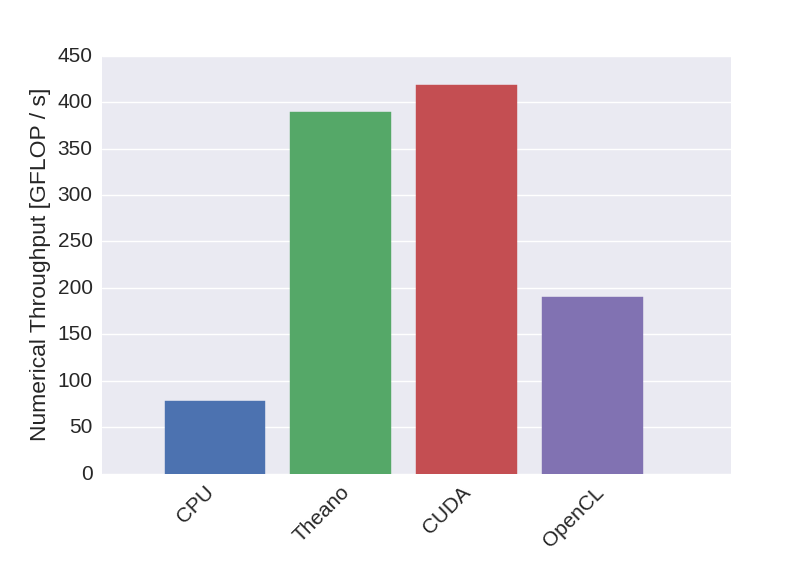
\includegraphics[width=0.8\linewidth]{results}
  \end{center}
\end{frame}
\section{Application to the Higgs Dataset}
\begin{frame}{The Higgs Dataset}
  \begin{itemize}
    \item \textbf{Signal Process}:
    \begin{flalign*}
      gg \rightarrow H^0 \rightarrow  W^\pm H^\mp
      \rightarrow W^\pm W^\mp h^0
       \rightarrow W^\pm W^\mp b\bar{b}
    \end{flalign*}
    \item \textbf{Background Process}:
    \begin{flalign*}
      gg \rightarrow t \bar{t} \rightarrow  W^\pm W^\mp b \bar{b}
    \end{flalign*}
    \item<2-> 21 \textbf{low-level features}: Momenta of one lepton and the four jets,
      jet b-tagging information, missing transverse momentum
    \item<2-> 7 \textbf{high-level features}: Derived invariant masses of
      intermediate decay products
    \item<2-> Dataset consisting of 11 million simulated collision events
    \end{itemize}
\end{frame}

\begin{frame}{Shallow vs. Deep Networks}
  \begin{itemize}
    \item \textbf{Shallow Network}: 1 hidden layer with $256$ neurons and $tanh$
      activation function and cross entropy loss
    \item \textbf{Deep Network}: 5 hidden layers with $256$ neurons and $tanh$
      activation function and cross entropy loss
    \item Both networks trained once using only low-level features and once using
      both high-level and low-level features.
 \end{itemize}
\end{frame}
\begin{frame}{Shallow vs. Deep Networks}
  \begin{center}
    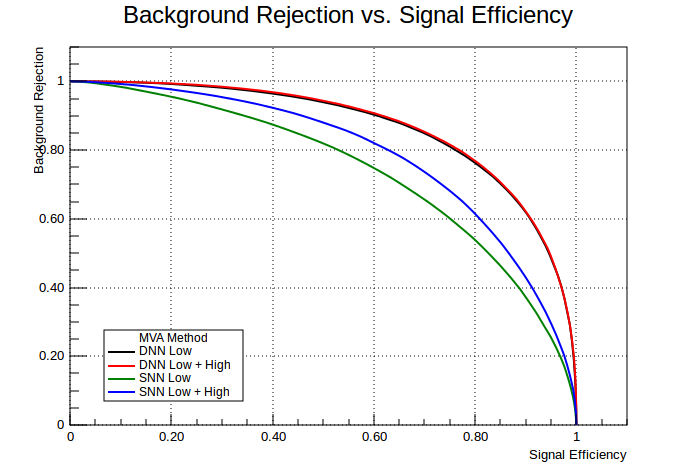
\includegraphics[width=0.8\linewidth]{dnn_low_high}
 \end{center}
\end{frame}
\begin{frame}{Deep Networks vs. BDT}
  \begin{itemize}
    \item \textbf{Deep Network}: 5 hidden layers with $256$ neurons and $tanh$
      activation function and cross entropy loss
    \item \textbf{Boosted Decision Trees}: 1000 Trees, maximum depth 3
    \item Both classifiers trained on low- and high-level features
 \end{itemize}
 \vskip 1cm
 \begin{center}
 \begin{tabular}{|l|c|c|}
   \hline
   Method & Training Time [h] & Area under ROC Curve \\
   \hline
   BDT & $4.78$ h & 0.806 \\
   DNN & $0.969$ h & 0.873 \\
   \hline
 \end{tabular}
 \end{center}
\end{frame}
\begin{frame}{Deep Networks vs. BDT}
  \begin{center}
    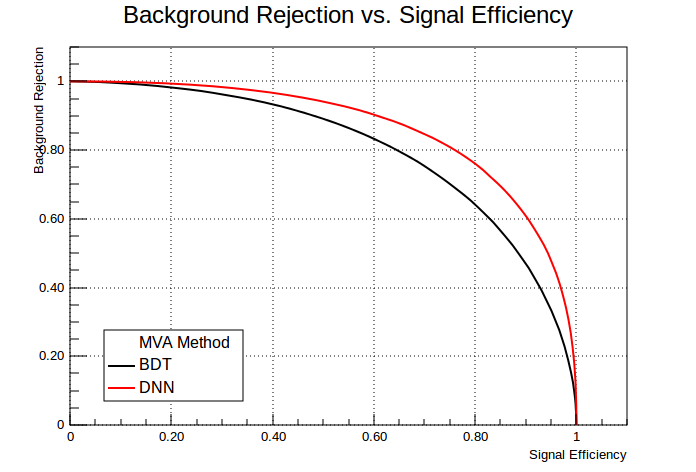
\includegraphics[width=0.8\linewidth]{bdt_dnn}
 \end{center}
\end{frame}

\section{Summary and Future Outlook}
\begin{frame}{Results}
  \begin{itemize}
    \item Testing and debugging of the prototype implementation
      of deep neural networks in TMVA.
    \item Production-ready implementation of parallel training
      of deep neural networks on CPUs and CUDA-capable GPUs.
    \item Reproduced Higgs benchmark results.
  \end{itemize}
\end{frame}
\begin{frame}{Future Outlook}
  \begin{itemize}
  \item \textbf{Near Future:}
    \begin{itemize}
    \item Integration of the CPU and CUDA
    \item Finish OpenCL implementation
    \end{itemize}
    \item Analyze performance on different architectures
    \item Extend neural network functionality: batch normalization, activation
      functions, AdaGrad, ...
  \end{itemize}
\end{frame}

\section{Acknowledgments}
\begin{frame}{Acknowledgments}
  \begin{itemize}
  \item Project carried out at \textbf{CERN} within the \textbf{Google Summer of Code}
    program
  \item \textbf{Supervisors}: Sergei V. Gleyzer, Lorenzo Moneta
  \end{itemize}
  \visible<2>{
    \begin{center}
      \huge Thank You!
    \end{center}
    }
    \begin{center}

\includegraphics[width=0.2\textwidth]{gsoc}%
\hskip 2cm 
\includegraphics[width=0.2\textwidth]{cern}
   \end{center}
\end{frame}
\end{document}


%%% Local Variables:
%%% mode: latex
%%% TeX-master: t
%%% End:
